% This include all the settings that we should use for the document
\newcommand{\PDFTitle}{DE10-Standard Computer System with ARM* Cortex* A9 Manual}
\newcommand{\commonPath}{../../../common/doc}
\newcommand{\templatePath}{../../../common/templates}
\newcommand{\sampleProgramsPath}{../../../sample_programs}
\input{\templatePath/defaulttext.tex}
\input{\templatePath/preamble.tex}

%%%%%%%%%%%%%%%%%%%%%%%%%
% Add title
\newcommand{\doctitle}{DE10-Standard Computer System\\ with ARM* Cortex* A9}
\newcommand{\dochead}{DE10-Standard Computer System with ARM* Cortex* A9}
% Usually no need to change these two lines
\title{\fontfamily{phv}\selectfont{\doctitle} }
\chead{ \small{\textsc{\bfseries \dochead} } }
% Customizations
\newcommand{\DEBoard}{DE10-Standard}
\newcommand{\systemName}{DE10-Standard Computer}
\newcommand{\systemNameFull}{DE10-Standard Computer with ARM A9}
\newcommand{\FPGADeviceFamily}{Cyclone\textsuperscript{\textregistered} V SoC}
\newcommand{\processor}{ARM A9}
\newcommand{\aProcessor}{an ARM A9}
\newcommand{\baseAddressOffset}{C}
\newcommand{\GIC}{GIC}
\newcommand{\videoOutDevice}{VGA}
\newcommand{\expansionPortA}{JP1}
\newcommand{\pixelBufferInfo}{320240_16}
\newcommand{\processorStyle}{defaultArmStyle}
\newcommand{\processorLower}{arm}
\clubpenalty 10000
\widowpenalty 10000
\raggedbottom
%%%%%%%%%%%%%%%%%%%%%%%%%

\begin{document}
\begin{table}
    \centering
    \begin{tabular}{p{5cm}p{4cm}}
        \hspace{-3cm}
        &
        \raisebox{1\height}{\parbox[h]{0.5\textwidth}{\Large\fontfamily{phv}\selectfont{\textbf{\doctitle}}}}
    \end{tabular}
    \label{tab:logo}
\end{table}

\colorbox[rgb]{0,0.384,0.816}{\parbox[h]{\textwidth}{\color{white}\textbf{\textit{\textBar}}}}

\thispagestyle{plain}

% Section: Introduction
\section{Introduction}
This document describes a computer system that can be implemented
on the \DEBoard~development and education board, which
is described in the \texttt{Teaching and Projects Boards} 
section of the {\small \href{https://www.fpgacademy.org/boards.html} {FPGAcademy.org}} website. 
This system, called the {\it \systemNameFull}, is intended for use in
experiments on computer organization and embedded
systems. 



% Section: Contents
\section{\systemName~Contents}
A block diagram of the \systemName~system is shown in 
Figure \ref{fig:block_diagram}.  As indicated in the figure, the components in this system 
are implemented utilizing the {\it Hard Processor System} (HPS) and FPGA 
inside the \FPGADeviceFamily~chip. The HPS comprises an ARM* Cortex* A9 dual-core 
processor, a DDR3 memory port, and a set of peripheral devices. The FPGA 
implements two Altera Nios\textsuperscript{\textregistered} processors, and several 
peripheral ports: memory, timer modules, 
audio-in/out, video-in/out, PS/2, analog-to-digital, infrared receive/transmit, and 
parallel ports connected to switches and lights.  Instructions for using the Nios processors
are provided in a separate document, called {\it \systemName~System with Nios II/V}.




\subsection{Hard Processor System}
\label{sec:hps}
The hard processor system (HPS), as shown in Figure~\ref{fig:block_diagram}, includes an 
ARM Cortex A9 dual-core processor. The A9 dual-core processor features two 32-bit CPUs 
and associated subsystems that are implemented as hardware circuits in the 
Cyclone V SoC chip.  An overview of the ARM A9 processor can be found in the 
document {\it Introduction to the ARM Processor}, which is 
available in the \texttt{Computer Organization System Design} section of the 
\href{https://www.fpgacademy.org/tutorials.html} {FPGAcademy.org} website.
All of the I/O peripherals in the \systemName~are
accessible by the processor as memory mapped devices, 
using the address ranges that are given in this document. A summary of the address map can
be found in Section {\ref{sec:mm}.

The easiest way to begin working with the \systemName~and the ARM processor is to use the
\href{https://cpulator.01xz.net/?sys=arm-de1soc} {CPUlator for {\it \systemNameFull}}.
The {\it CPUlator} is a powerful and easy-to-use functional simulator that runs inside a
web browser. It simulates the behavior of a whole computer system, including the
processor, memory, and many types of I/O devices. The CPUlator simulator supports a variety
of different computer systems, including the {\it \systemNameFull}. 
The CPUlator user interface displays all of the information that a programmer needs to
develop and debug software code running on the {\it \systemNameFull}. It shows (and allows
you to edit) the values in the processor general-purpose and control registers, as well as the 
contents of memories in the computer system and the values of memory-mapped I/O device 
registers. The CPUlator allows software code, written either in assembly language or the 
C language, to be entered into the simulator, assembled to produce machine code, loaded 
into memory, and then executed. The user can set breakpoints in the machine code, 
single-step instructions, and perform any of the usual operations that are supported in 
typical debugging environments.

A good way to develop software code that runs on the actual \systemNameFull~hardware
is to make use of a utility called the {\it \productNameMed{}}.  It
provides an easy way to assemble/compile ARM A9 programs written in either assembly language or 
the C language. The Monitor Program, which can be downloaded from 
the \href{https://www.fpgacademy.org/tools.html} {FPGAcademy.org} website, is 
an application program that runs on the host computer connected to the \DEBoard~board.  
The Monitor Program can be used to control the execution of code on the ARM A9, list (and edit) 
the contents of processor registers, display/edit the contents of memory on the \DEBoard~
board, and similar operations.  The Monitor Program includes the \systemName~as a 
pre-designed system that can be downloaded onto the \DEBoard~board, as well as several sample 
programs in assembly language and C that show how to use the \systemName's peripherals.
Section~\ref{sec:monitor_program} describes how the \systemName~is integrated with the 
Monitor Program.


\begin{figure}[h!]
   \begin{center}
        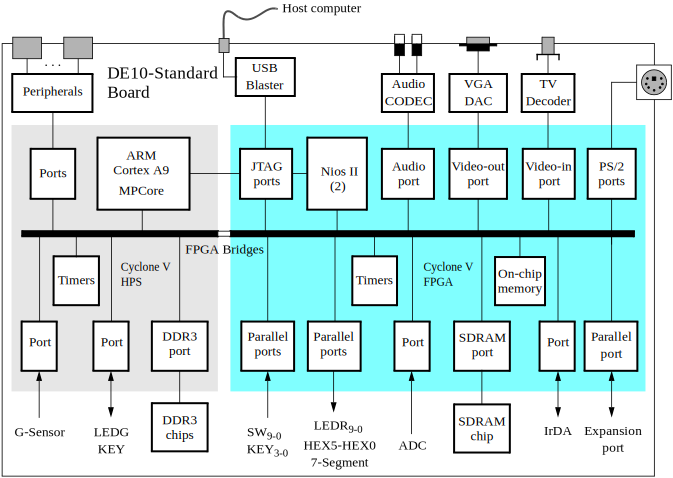
\includegraphics[height=.4\paperheight]{../common/figures/fig_block_diagram.png}
   \end{center}
   \caption{Block diagram of the \systemName.}
	\label{fig:block_diagram}
\end{figure}


\subsection{Memory}
\label{sec:ddr3}
The HPS includes a memory port that connects the ARM MPCORE* to a 1 GB DDR3 memory.
This memory is normally used as the storage location of programs and data used by the ARM
processors. The memory is organized as 256M {\sf x} 32-bits, and is accessible using word
accesses (32 bits), halfwords, and bytes. The DDR3 memory is mapped to the address space
{\sf 0x00000000} to {\sf 0x3FFFFFFF}. There is also a 64 KB on-chip memory available inside 
each ARM A9 processor. This small memory is organized as 16K {\sf x} 32-bits, and is mapped 
to the address space {\sf 0xFFFF0000} to {\sf 0xFFFFFFFF}.


\subsection{Pushbutton KEY and LED Port}
\label{sec:hps_gpio1}
The HPS includes a general purpose I/O port, called {\it GPIO1}, that is accessible by the
ARM A9 processor.  As illustrated in Figure~\ref{fig:gpio1}, this parallel 
port is assigned the {\it Base} address {\sf 0xFF709000}, and includes several 32-bit registers.
These registers can be read or written using word accesses.
Only two bit locations in GPIO1 are used for the \systemName. Bit~24 of the data
register (DR) is connected to
a green light, LEDG, and bit~25 is connected to a pushbutton switch, KEY. To use these
devices, the {\it data direction register} (DDR) shown in the figure has to be configured such 
that bit~24 is an output and bit~25 is an input. Writing a 1 into a corresponding bit
position in the DDR sets this bit as an output, while writing a 0 sets the bit as an
input. After the direction bits have been set, the green light LEDG can be turned on/off 
by writing to bit~24 in the data register. The
value of the pushbutton switch KEY can be obtained by reading the external port register
and checking the value 
of bit~25. An example program for the ARM A9 processor that uses GPIO1 is given in Section
\ref{sec:timers}.

As indicated in Figure~\ref{fig:gpio1}, the GPIO1 port includes several other registers in
addition to the DR and DDR registers. These other registers are mostly used for setting
characteristics of input pins, which affects only the KEY input in our system.
Detailed information about these registers can be found in the {\it Cyclone V Hard 
Processor System} documentation, which is available on the Internet.

\begin{figure}[h!]
   \begin{center}
       \includegraphics{../../../common/figs/HPS_GPIO1.pdf}
   \end{center}
   \caption{Parallel port GPIO1.}
	\label{fig:gpio1}
\end{figure}

\subsection{Timer Modules}
\label{sec:timers}
The HPS includes several hardware timer modules that can be used to keep track of time intervals.
The ARM A9 MPCore includes one {\it private} timer module for each A9 core, and the
HPS provides four other timer modules that can be used by either A9 core. The timers are 
described in more detail below.

\subsubsection{ARM* A9* MPCore* Timers}
\label{sec:ARM_timers}
Figure~\ref{fig:MPCORE_timer} shows the registers in the programmer's interface for each
A9 core private timer. These registers have the base address {\sf 0xFFFEC600}, as shown in
the figure, and can be read or written using word accesses. To use the timer, 
it is necessary to first write an
initial count value into the {\it Load} register. The timer can then be started by
setting the enable bit $E$ in the {\it Control} register to 1, and it can be stopped by
setting $E$ back to 0.  Once enabled the timer decrements its count value until reaching 0.
When it reaches 0, the timer sets the {\it F} bit in the {\it Interrupt status} register. 
The {\it F} bit can be checked by software using polled-I/O to determine when the timer
period has expired.  The {\it F} bit can be reset to 0 by writing a 1 into it. 
Also, if bit~{\it I} in the {\it Control} register is set to 1,
then a processor interrupt can be generated when the timer reaches 0.  Using 
interrupts with the timer is discussed in Section~\ref{sec:exceptions}.

When it reaches 0, the timer will stop if the auto bit ({\it A}) in the control register
is set to 0.  But if bit {\it A} is set to 1, then the timer will automatically reload the 
value in the {\it Load} register and continue decrementing. The current value of the timer is
available to software in the {\it Counter} register shown in Figure~\ref{fig:MPCORE_timer}.
The timer uses a clock frequency of 200 MHz. The {\it Prescaler} field in the {\it
Control} register can be used to slow down the counting rate, as follows. The timer decrements 
each {\it Prescaler} $+1$ clock cycle. Therefore, if {\it Prescaler} $=0$, then the
timer decrements every clock cycle, if {\it Prescaler} $=1$, the timer
decrements every second clock cycle, and so on.

\begin{figure}[h!]
   \begin{center}
       \includegraphics{../../../common/figs/HPS_MPCORE_Timer.pdf}
   \end{center}
   \caption{ARM A9 private timer port.}
	\label{fig:MPCORE_timer}
\end{figure}

\subsubsection{HPS Timers}
\label{sec:HPS_timers}
Figure~\ref{fig:HPS_timer} shows the registers in the programmer's interface for one of 
the HPS timers.  These registers have the base address {\sf 0xFFC08000}, as shown in
the figure, and can be read or written using word accesses. To configure the timer, 
it is necessary to ensure that it is stopped by setting the enable bit $E$ 
in the {\it Control} register to 0. A starting count value for the timer can then be written into
the {\it Load} register. To instruct the timer to use the specified starting count value, the
{\it M} in the {\it Control} register should be set to 1, and the timer can be started by 
setting $E = 1$. The timer counts down to 0, and then sets both bit $F$ in the 
{\it End-of-interrupt} register and bit {\it S} in the {\it Interrupt status} register to 1. 
Software can poll the value of $S$ to determine when the timer period has expired. 
The {\it S} bit, and the {\it F} bit can be reset to 0 by reading the contents of 
the {\it End-of-Interrupt} register.  Also, if bit $I$, the interrupt mask bit, in 
the {\it Control} register is set to 0, then an interrupt can be generated when 
the timer reaches 0 (note that bit {\it I} in the ARM A9 private timer shown in 
Figure~\ref{fig:MPCORE_timer} has the opposite polarity). The use of interrupts with the
timer is discussed in Section~\ref{sec:exceptions}.

The current value of the timer is available to software in the {\it Counter} register shown in 
Figure~\ref{fig:HPS_timer}.  The timer uses a clock frequency of 100 MHz. 

There are three other identical timers in the HPS, with the following base
addresses: {\sf 0xFFC09000}, {\sf 0xFFD00000}, and {\sf 0xFFD01000}. The first of these
timers uses a 100 MHz clock, and the last two timers use a 25 MHz clock.

We should mention that other timer modules also exist in the HPS. The ARM A9 MPCore has
a {\it global} timer that is shared by both A9 cores, as well as a {\it watchdog} timer
for each processor. Also, the HPS has two additional watchdog timers. Documentation about
the global timer and watchdog timers is available in the {\it ARM Cortex A9 MPCore
Technical Reference Manual}, and in the {\it Cyclone V Hard Processor System
Technical Reference Manual}.

\begin{figure}[h]
   \begin{center}
       \includegraphics{../../../common/figs/HPS_Timer.pdf}
   \end{center}
   \caption{HPS timer port.}
	\label{fig:HPS_timer}
\end{figure}

\subsubsection{Using a Timer with Assembly Language Code}
\label{sec:ARM_assembly}
An example of ARM A9 assembly language code is included in the Appendix in Listing~\ref{lst:timer_s}. The code 
configures the private timer for the A9 core so that it produces one-second timeouts. An
infinite loop is used to flash the green light connected to GPIO1, discussed
in Section \ref{sec:hps_gpio1}. The light is turned on for one second, then off, and so on.

An example of C code is also included in Listing~\ref{lst:timer_C}. This code performs the same actions 
as the assembly language program in Listing~\ref{lst:timer_s}---it flashes on/off the green 
light connected to GPIO1 at one-second intervals.

The source code files shown in Listings~\ref{lst:timer_C} and~\ref{lst:timer_s}
are distributed as part of the  
\productNameMed{}. The files can be found under the heading {\it sample programs}, 
and are identified by the name {\it Timer Lights}.



\subsection{FPGA Bridges}
\label{sec:FPGA_bridge}
The {\it FPGA bridges} depicted in Figure~\ref{fig:block_diagram} provide connections between
the HPS and FPGA in the Cyclone V SoC device. The bridges are enabled, or disabled, 
by using the {\it Bridge reset} register, which is illustrated in 
Figure~\ref{fig:FPGA_bridge} and has the address {\sf 0xFFD0501C}.  
Three distinct bridges exist, called {\it HPS-to-FPGA}, {\it lightweight HPS-to-FPGA}, and 
{\it FPGA-to-HPS}.  In the \systemName~the first two of these bridges are used to
connect the ARM A9 processor to the FPGA.  As indicated in 
Figure~\ref{fig:FPGA_bridge} the bridges are enabled/disabled by bits $0-2$ of the 
{\it Bridge reset} register.  To use the memory-mapped peripherals in the FPGA, software 
running on the ARM A9 must enable the HPS-to-FPGA and lightweight HPS-to-FPGA bridges by
setting bits \#0 and \#1 of the {\it Bridge reset} register to 0. 
We should note that if a user program is downloaded and run on the ARM A9 by using the
\productNameMed{}, described in Section~\ref{sec:monitor_program},
then these bridges are automatically enabled before the user program is started.

\begin{figure}[h!]
   \begin{center}
       \includegraphics{../../../common/figs/HPS_FPGA_Bridges.pdf}
   \end{center}
   \caption{FPGA bridge reset register.}
	\label{fig:FPGA_bridge}
\end{figure}

In addition to the components described above, the HPS also provides a number of other
peripheral devices, such as USB, Ethernet, and a 3-D accelerometer (G-sensor). The
G-sensor is described in the tutorial {\it Using the Accelerometer on DE-series Boards}, 
which is available in the \texttt{Hardware Components} section of the
\href{https://www.fpgacademy.org/tutorials.html} {FPGAcademy.org} website.
Documentation about the other devices 
connected to the HPS can be found in the {\it Cyclone V Hard Processor System
Technical Reference Manual}, as well as in the {\it \DEBoard~Board User Manual}.



\subsection{G-Sensor}
\label{sec:hps_gsensor}
The \systemName~includes a 3D accelerometer (G-sensor) that is connected to the HPS. The accelerometer can be configured to produce two interrupt signals. One of
these signals is
used in our system and is connected to an I/O port on the HPS called GPIO2.
This I/O port has the same structure as GPIO1 which was described in Section \ref{sec:hps_gpio1}. The base address of GPIO2 is {\sf 0xFF70A000}. The accelerometer interrupt signal
is connected to bit 5 in the data register of GPIO2. 
The accelerometer generates an interrupt by driving
the interrupt signal high. The "interrupt"
signal is not connected to the generic interrupt controller (GIC) of the HPS, so to
check for interrupts the bit must be polled.

\subsection{FPGA Components}
\label{sec:fpga}
As shown in Figure \ref{fig:block_diagram} a number of components in the \systemName~are 
implemented inside the FPGA in the \FPGADeviceFamily~chip.  Several of these components 
are described in this section, and the others are presented in Section~\ref{sec:multi}.

\subsection{Nios\textsuperscript{\textregistered} II Processor}
\label{sec:nios2}
The Nios II processor is a 32-bit CPU that can be implemented
in an Altera FPGA device.  Two versions of the Nios II processor are available,
designated economy (/e) and fast (/f). The \systemName~includes two instances of the Nios II/f version, configured with floating-point hardware 
support.

Instructions for using the Nios II processors in the \systemName~are provided in 
a separate document, called {\it \systemName~with Nios II}.


\subsection{Memory Components}
The \systemName~has an SDRAM port, as well as two memory modules implemented using the 
on-chip memory inside the FPGA. These memories are described below.

\subsubsection{SDRAM}
An SDRAM Controller in the FPGA provides an interface to the 64 MB synchronous dynamic RAM (SDRAM) 
on the \DEBoard~board, which is organized as 32M {\sf x} 16 bits. It is
accessible by the \processor~processor using word (32-bit), halfword (16-bit), or byte
operations, and is mapped to the address space {\sf 0x\baseAddressOffset 0000000} to {\sf 0x\baseAddressOffset 3FFFFFF}.



\subsubsection{On-Chip Memory}
A 256 KB memory is implemented inside the FPGA, organized as 64K {\sf x} 32 bits. The 
{\processor} processor can access this memory using addresses in the range 
{\sf 0x\baseAddressOffset 8000000} to {\sf 0x\baseAddressOffset 803FFFF}. This
memory is used as a pixel buffer for the video-out and video-in ports.


\subsubsection{On-Chip Memory Character Buffer}
An 8 KB memory is implemented inside the FPGA for use as a character buffer for the video-out
port, which is described in Section~\ref{sec:video_out}.
The character buffer memory is organized as 8K {\sf x} 8 bits, and spans the {\processor}
address range {\sf 0x\baseAddressOffset 9000000} to {\sf 0x\baseAddressOffset 9001FFF}.



\subsection{Parallel Ports}
There are several parallel ports implemented in the FPGA that support input, output, and
bidirectional transfers of data between the \processor~processor and I/O peripherals. As 
illustrated in Figure~\ref{fig:parallel_port}, each parallel port is assigned a {\it Base}
address and contains up to four 32-bit registers. Ports that have output capability include a
writable {\it Data} register, and ports with input capability have a readable {\it
Data} register. Bidirectional parallel ports also include a {\it Direction} register that 
has the same bit-width as the {\it Data} register. Each bit in the {\it Data} register can be
configured as an input by setting the corresponding bit in the {\it Direction} register to 0,
or as an output by setting this bit position to~1. The {\it Direction} register is assigned the
address {\it Base} + 4.

\begin{figure}[h!]
   \begin{center}
       \includegraphics{../../../common/figs/FPGA_PP.pdf}
   \end{center}
   \caption{Parallel port registers in the {\it \systemNameFull}.}
	\label{fig:parallel_port}
\end{figure}

Some of the parallel ports have registers at addresses 
{\it Base} + 8 and {\it Base} + C, as indicated in Figure~\ref{fig:parallel_port}. These
registers are discussed in Section \ref{sec:exceptions}.



\subsubsection{Red LED Parallel Port}

The red lights {\it LEDR}$_{9-0}$ on the \DEBoard~board
are driven by an output parallel port, as illustrated in Figure \ref{fig:LED_port}. The port
contains a 10-bit {\it Data} register, which has the
address {\sf 0xFF200000}.  This register can be written or read by the processor using word 
accesses, and the upper bits not used in the registers are ignored.

\begin{figure}[h!]
   \begin{center}
       \includegraphics{../../../common/figs/FPGA_PP_Red_LEDs_10.pdf}
   \end{center}
   \caption{Output parallel port for {\it LEDR}.}
	\label{fig:LED_port}
\end{figure}



\subsubsection{7-Segment Displays Parallel Port}

There are two parallel ports connected to the 7-segment displays on the \DEBoard~board, each of
which comprises a 32-bit write-only {\it Data} register. As indicated in 
Figure \ref{fig:hex_segment_port}, the register at address {\sf 0xFF200020} 
drives digits {\it HEX3} to {\it HEX0}, and the register at 
address {\sf 0xFF200030} drives digits {\it HEX5} and
{\it HEX4}.  Data can be written into these two registers, and read back, by using word operations. 
This data directly controls the segments of each display, according to
the bit locations given in Figure \ref{fig:hex_segment_port}. The locations of segments 
6 to 0 in each seven-segment display on the \DEBoard~board is illustrated on the right side of the
figure.

\begin{figure}[h!]
   \begin{center}
       \includegraphics{../../../common/figs/FPGA_PP_7_Segs_6.pdf}
   \end{center}
   \caption{Bit locations for the 7-segment displays parallel ports.}
	\label{fig:hex_segment_port}
\end{figure}


\subsubsection{Slider Switch Parallel Port}

The {\it SW}$_{9-0}$ slider switches on the \DEBoard~board are connected to an input parallel
port.  As illustrated in Figure~\ref{fig:slider_port}, this port 
comprises a 10-bit read-only {\it Data} register, which is mapped to address {\sf 0xFF200040}.

\begin{figure}[h!]
   \begin{center}
       \includegraphics{../../../common/figs/FPGA_PP_Switches_10.pdf}
   \end{center}
   \caption{{\it Data} register in the slider switch parallel port.}
	\label{fig:slider_port}
\end{figure}


\input{\commonPath/FPGA_PP_Keys_4.tex}

\subsubsection{Expansion Parallel Port}

The \systemName~includes one bidirectional parallel port that is connected to the
{\it \expansionPortA} expansion header on the \DEBoard~board. This parallel port
includes the four 32-bit registers that were described previously for 
Figure~\ref{fig:parallel_port}. The base address of this port is {\sf 0xFF200060}.
Figure \ref{fig:expansion_port} gives a diagram of 
the {\it JP1} expansion connector on the \DEBoard~board, and shows how the respective parallel port {\it Data} register bits, 
$D_{31-0}$, are assigned to the pins on the connector. The figure shows that bit $D_0$ of
the parallel port is assigned to the pin at the top right corner of the
connector, bit $D_1$ is assigned below this, and so on. Note that some of the pins on
{\it \expansionPortA} are not usable as input/output connections, and are 
therefore not used by the parallel ports. Also, only 32 of the 36 data pins that appear on
each connector can be used.

\begin{figure}[h!]
   \begin{center}
       \includegraphics[trim={0 0 0 0.5cm},clip]{../../../common/figs/FPGA_PP_Expansion_Port_Single.pdf}
   \end{center}
   \caption{Assignment of parallel port bits to pins.}
	\label{fig:expansion_port}
\end{figure}
\input{\commonPath/FPGA_PP_Examples.tex}

\subsection{JTAG* Port}
\label{sec:jtag_port}

The JTAG* port implements a communication link between the \DEBoard~board and its host computer.  
This link can be used by the Quartus\textsuperscript{\textregistered} Prime software to transfer FPGA programming files 
into the \DEBoard~board, and by the \productNameMed{}, discussed in 
Section~\ref{sec:monitor_program}.  The JTAG port also
includes a UART, which can be used to transfer character data between the host computer and
programs that are executing on the \processor~processor.
The programming interface 
of the JTAG UART consists of two 32-bit registers, as shown in Figure \ref{fig:jtag_port}. 
The register mapped to address {\sf 0xFF201000} is called the {\it Data}
register and the register mapped to address {\sf 0xFF201004} is called the {\it Control}
register.

\begin{figure}[h!]
   \begin{center}
       \includegraphics{../../../common/figs/FPGA_JTAG_UART.pdf}
   \end{center}
   \caption{JTAG UART registers.}
	\label{fig:jtag_port}
\end{figure}

When character data from the host computer is received by the JTAG UART 
it is stored in a 64-character FIFO.  The number of characters currently stored in this FIFO is
indicated in the field {\it RAVAIL}, which are
bits 31$-$16 of the {\it Data} register.  If the receive FIFO overflows, then
additional
data is lost. When data is present in the receive FIFO, then the value of {\it RAVAIL} will be 
greater than 0 and the value of bit 15, {\it RVALID}, will be 1. Reading the character at
the head of the FIFO, which is provided in bits $7-0$, decrements the value of {\it RAVAIL} 
by one and returns this decremented value as part of the read
operation. If no data is present in the receive FIFO, then {\it RVALID} will 
be set to 0 and the data in bits $7-0$ is undefined.

The JTAG UART also includes a 64-character FIFO that stores data 
waiting to be transmitted to the host computer. 
Character data is loaded into this FIFO by performing a write to bits 7$-$0
of the {\it Data} register in Figure \ref{fig:jtag_port}.  
Note that writing into this register has no effect 
on received data.  The amount of space, {\it WSPACE}, currently available in the transmit FIFO is 
provided in bits 31$-$16 of the {\it Control} register.  If
the transmit FIFO is full, then any characters written to the {\it Data} register will be lost.

Bit 10 in the {\it Control} register, called {\it AC}, has the value 1 if the JTAG UART has been
accessed by the host computer. This bit can be used to check if a working connection to
the host computer has been established. The {\it AC} bit can be cleared to 0 by writing a 1
into it.

The {\it Control} register bits {\it RE}, {\it WE}, {\it RI}, and {\it WI} are described 
in Section \ref{sec:exceptions}.

\subsubsection{Using the JTAG* UART with Assembly Language Code and C Code}

Listings \ref{lst:jtag_uart_s} and \ref{lst:jtag_uart_C} give simple examples of 
assembly language and C code, respectively, that use the JTAG UART. Both versions of the
code perform the same function, which is to first send an ASCII string to the JTAG UART,
and then enter an endless loop. In the loop, the code reads character data that has 
been received by the JTAG UART, and echoes this data back to the UART for transmission. In
the {\it CPUlator} simulator, there is a JTAG window that allows text to be typed and
echoed. If the program is executed by using the \productNameMed{}, then any keyboard character that 
is typed into the {\it Terminal Window} of the Monitor Program will be 
echoed back, causing the character to appear in the {\it Terminal Window}.

The source code files shown in Listings \ref{lst:jtag_uart_s} and \ref{lst:jtag_uart_C}
are made available as part of the  
\productNameMed{}. The files can be found under the heading {\it sample programs}, 
and are identified by the name {\it JTAG UART}.


\subsubsection{Second JTAG* UART}

The \systemName~includes a second JTAG UART that is accessible by the ARM A9 MPCORE.
This second UART is mapped to the base address {\sf 0xFF201008}, and operates as described
above. The reason that two JTAG UARTs are provided is to allow each processor in the ARM
A9 MPCORE to have access to a separate UART.


\subsection{Interval Timers}
\label{sec:interval_port}

The {\it \systemNameFull} includes a timer module implemented in the FPGA that can be used by
the \processor~processor. This timer can be loaded with a preset value, and then counts down to 
zero using a 100-MHz clock. The programming interface 
for the timer includes six 16-bit registers, as illustrated in Figure~\ref{fig:interval_port}.  
The 16-bit register at address {\sf 0xFF202000} provides status information about the timer,
and the register at address {\sf 0xFF202004} allows control settings to be made.  The bit 
fields in these registers are described below:

\begin{itemize}
\item
{\it TO} provides a timeout signal which is set to 1 by the timer when it 
has reached a count value of zero.  The {\it TO} bit can be reset by writing a 0 into it. 
\item 
{\it RUN} is set to 1 by the timer whenever it is currently counting. Write 
operations to the status halfword do not affect the value of the {\it RUN} bit. 

\item 
{\it ITO} is used for generating interrupts, which are discussed in section \ref{sec:exceptions}.

\begin{figure}[h!]
   \begin{center}
       \includegraphics{../../../common/figs/FPGA_Interval_Timers.pdf}
   \end{center}
   \caption{Interval timer registers.}
	\label{fig:interval_port}
\end{figure}

\item
{\it CONT} affects the continuous operation of the timer.  When the timer reaches
a count value of zero it automatically reloads the specified starting count value. If 
{\it CONT} is set to 1, then the timer will continue counting down automatically.
But if {\it CONT} $=0$, then the timer will stop after it has reached a count value of 0. 

\item
({\it START}/{\it STOP}) is used to commence/suspend the operation of the 
timer by writing a 1 into the respective bit.
\end{itemize}

The two 16-bit registers at addresses {\sf 0xFF202008} and {\sf 0xFF20200C}
allow the period of the timer to be changed by
setting the starting count value.  The default setting gives a timer period of 125 msec. 
To achieve this period, the starting value of the count is
100 MHz $\times$ 125 msec $=12.5\times10^6$. It is possible to capture a snapshot of the 
counter value at any time by performing a write to address {\sf 0xFF202010}. This write
operation causes the current 32-bit counter value to be stored into the two 16-bit timer
registers at addresses {\sf 0xFF202010} and {\sf 0xFF202014}. These registers can then be
read to obtain the count value.

A second interval timer, which has an identical interface to the one described above, is also 
available in the FPGA, starting at the base address {\sf 0xFF202020}.


\subsection{System ID}

The system ID module provides a unique value that identifies the \systemName~
system.  The host computer connected to the \DEBoard~board can query the
system ID module by performing a read operation through the JTAG port. The host computer can 
then check the value of the returned identifier to confirm that the \systemName~has 
been properly downloaded onto the \DEBoard~board.  This process allows debugging tools on the 
host computer, such as the \productNameMed{}, to verify that the 
\DEBoard~board contains the required computer system before attempting to execute code 
that has been compiled for this system.


% Section: Exceptions and Interrupts
\section{Exceptions and Interrupts}
\label{sec:exceptions}

The A9 processor supports eight types of exceptions, including the {\it reset} exception and the
{\it interrupt request} (IRQ) exception, as well a number of exceptions related to 
error conditions. All of the exception types are described in the document 
{\it Introduction to the ARM Cortex-A9 Processor}, which is provided in 
the \texttt{Computer Organization System Design} section of the 
\href{https://www.fpgacademy.org/tutorials.html} {FPGAcademy.org} website.
Exception processing uses a table in memory, called the {\it vector table}. This 
table comprises eight words in memory and has one entry for each type of exception. The 
contents of the vector table have to be set up by software, which typically places a 
branch instruction in each word of the table, where the branch target is the desired 
exception service routine. When an exception occurs, the ARM processor stops the 
program that is currently running, and then fetches the instruction 
stored at the corresponding vector table entry.  The vector table usually starts at 
the address {\sf 0x00000000} in memory. The first entry in the table corresponds to the 
reset vector, and the IRQ vector uses the seventh entry in the table, at the 
address {\sf 0x00000018}.

The IRQ exception allows I/O peripherals to generate interrupts for the A9 processor.
All interrupt signals from the peripherals are connected to a module in the processor
called the {\it Generic Interrupt Controller} (GIC). The GIC allows individual interrupts
for each peripheral to be either enabled or disabled. When an enabled interrupt happens, the 
GIC causes an IRQ exception in the A9 processor. Since the same vector table entry is used for 
all interrupts, the software for the interrupt service routine must determine the source 
of the interrupt by querying the GIC. Each peripheral is identified in the GIC by an
interrupt identification (ID) number.  Table \ref{tab:irq}
gives the assignment of interrupt IDs for each of the I/O peripherals in the \systemName.
The rest of this section describes the interrupt behavior associated with the 
timers and parallel ports.



\begin{table}[h]
    \begin{center}
    \begin{tabular}{l|c}
          \textbf{I/O Peripheral} &
          \textbf{Interrupt ID \#}        \\
          \hline\vspace{-3mm}             \\
          A9 Private Timer & 29           \\
          HPS GPIO1 & 197                 \\
          HPS Timer 0 & 199               \\
          HPS Timer 1 & 200               \\
          HPS Timer 2 & 201               \\
          HPS Timer 3 & 202               \\
		  FPGA Interval Timer & 72        \\
		  FPGA Pushbutton KEYs & 73       \\
		  FPGA Second Interval Timer & 74 \\
		  FPGA Audio & 78                 \\
		  FPGA PS/2 & 79                  \\
		  FPGA JTAG & 80                  \\
		  FPGA Infrared (IrDA) & 81       \\
		  FPGA JP1 Expansion & 83         \\
		  FPGA PS/2 Dual & 89             \\
    \end{tabular}
    \caption{Interrupt IDs in the \systemName.}
	\label{tab:irq}
    \end{center}
\end{table}

\subsection{Interrupts from the ARM* A9* Private Timer}

Figure~\ref{fig:MPCORE_timer}, in Section~\ref{sec:ARM_timers}, shows four registers that
are associated with the A9 private timer. As we said in Section \ref{sec:ARM_timers}, bit
{\it F} in the {\it Interrupt status} register is set to 1 when the timer reaches a count 
value of 0. It is possible to generate an A9 interrupt when this occurs, by using bit {\it I}
of the {\it Control} register.  Setting bit {\it I} to 1 causes the timer to send an
interrupt signal to the GIC whenever the timer reaches a count value of 0. 
The {\it F} bit can be cleared to 0 by writing writing a 1 into the 
{\it Interrupt status} register.



\subsection{Interrupts from the HPS Timers}

Figure~\ref{fig:HPS_timer}, in Section~\ref{sec:HPS_timers}, shows five registers that
are associated with each HPS timer. As we said in Section \ref{sec:HPS_timers}, 
when the timer reaches a count value of zero, bit~{\it F} in the {\it End-of-Interrupt} register 
is set to 1. The value of the {\it F}~bit is also reflected in the {\it S}~bit in the 
{\it Interrupt status} register.  It is possible to generate an A9 interrupt when the 
{\it F}~bit becomes 1, by using the {\it I}~bit of the {\it Control} register.  
Setting bit {\it I} to 0 {\it unmasks} the interrupt signal, and causes the timer to send an
interrupt signal to the GIC whenever the {\it F}~bit is 1.  After an interrupt occurs, it can 
be cleared by reading the {\it End-of-Interrupt} register.



\subsection{Interrupts from the FPGA Interval Timer}

Figure \ref{fig:interval_port}, in Section \ref{sec:interval_port}, shows six registers that
are associated with the interval timer. As we said in Section \ref{sec:interval_port}, the
{\it TO}~bit in the {\it Status} register is set to 1 when the timer reaches a count value of 0.
It is possible to generate an interrupt when this occurs, by using the {\it ITO}~bit in 
the {\it Control} register. Setting the {\it ITO}~bit to 1 causes an interrupt request to 
be sent to the \GIC~whenever {\it TO} becomes 1. After an interrupt occurs, it can be cleared 
by writing any value into the {\it Status} register.




\subsection{Interrupts from Parallel Ports}

Parallel ports were illustrated in Figure~\ref{fig:parallel_port}, which is reproduced 
as Figure~\ref{fig:parallel_port_int}.
As the figure shows, parallel ports that support interrupts include two related registers 
at the addresses {\it Base} + 8 and {\it Base} + C.
The {\it Interruptmask} register, which has the address {\it Base} + 8, specifies whether 
or not an interrupt signal should be sent to the \GIC~when the data present at
an input port changes value.  Setting a bit location in this register to 1 allows 
interrupts to be generated, while setting the bit to 0 prevents interrupts. 
Finally, the parallel port may contain an {\it Edgecapture} register at address
{\it Base} + C.  Each bit in this register has the value 1 if the 
corresponding bit location in the parallel port has changed its value from 0 to 1.
A bit in the {\it Edgecapture} register can be cleared to 0
by writing a 1 into the corresponding bit position, which clears any associated interrupt. 

\begin{figure}[h!]
   \begin{center}
       \includegraphics{../../../common/figs/Interrupts_FPGA_PP.pdf}
   \end{center}
   \caption{Registers used for interrupts from the parallel ports.}
	\label{fig:parallel_port_int}
\end{figure}



\subsubsection{Interrupts from the Pushbutton KEY Port}

Figure \ref{fig:pushbutton_port}, reproduced as Figure \ref{fig:pushbutton_port_int},
shows the registers associated with the pushbutton KEY port. 
The {\it Interruptmask} register allows interrupts to be generated when a key is
pressed. Interrupts can be enabled individually for each key by setting its 
{\it Interruptmask} bit to 1.  When a key is pressed, the corresponding bit in the 
{\it Edgecapture} register is set to 1 by the parallel port. This bit remains 1
until cleared to 0 by software.  An interrupt service routine can read the {\it Edgecapture} 
register to determine which key/s has/have been pressed.  An {\it Edgecapture} register bit can 
be cleared by writing a logic value 1 into the bit position.  Clearing the
bit resets the corresponding interrupt signal being sent to the \GIC.

\begin{figure}[h!]
   \begin{center}
       \includegraphics{../../../common/figs/FPGA_PP_Keys.pdf}
   \end{center}
   \caption{Registers used for interrupts from the pushbutton KEY port.}
	\label{fig:pushbutton_port_int}
\end{figure}


\subsection{Interrupts from the JTAG* UART}

Figure \ref{fig:jtag_port}, reproduced as Figure \ref{fig:jtag_port_int}, shows the {\it Data} 
and {\it Control} registers of the JTAG UART. As we said in Section~\ref{sec:jtag_port}, 
{\it RAVAIL} in the {\it Data} register gives the number of characters that 
are stored in the receive 
FIFO, and {\it WSPACE} gives the amount of unused space that is available in the transmit FIFO. 
The {\it RE} and {\it WE} bits in Figure \ref{fig:jtag_port_int}
are used to enable processor interrupts associated with the receive and transmit FIFOs. 
When enabled, interrupts are generated when {\it RAVAIL} for the receive FIFO, 
or {\it WSPACE} for the transmit FIFO, exceeds 7. Pending interrupts are indicated in the 
Control register's {\it RI} and {\it WI} bits, and can be cleared by writing or reading data
to/from the JTAG UART.

\begin{figure}[h!]
   \begin{center}
       \includegraphics{../../../common/figs/FPGA_JTAG_UART.pdf}
   \end{center}
   \caption{Interrupt bits in the JTAG UART registers.}
	\label{fig:jtag_port_int}
\end{figure}




\subsection{Using Interrupts with Assembly Language Code}

An example of assembly language code for the \systemName~that uses interrupts is
shown in Listing \ref{lst:interrupt_example_s}, which has three main parts. The beginning
part of the code 
sets up the exception vector table. This code must be in a special assembler section called
.{\bf section}, as shown.  The entries in the table provide branches
to the various exception service routines; they are discussed later in this section.

When this code is executed on the \DEBoard~board
it displays a rotating pattern on the LEDs. The pattern's rotation can be toggled through pressing the pushbutton KEYs.
Different types of interrupts are used in the code. The LEDs are controlled by interrupts from the FPGA
interval timer, and the KEYs are also handled through interrupts.

The main program initializes the A9 banked stack pointer (sp) registers for interrupt (IRQ) mode 
and supervisor (SVC) mode, because these are the processor modes that are
used in the program. The code then calls subroutines to initialize the HPS timer, FPGA
interval timer, and FPGA pushbutton KEYs. Finally, the code initializes the HPS GPIO1
port, enables IRQ interrupts in the A9 processor, and then enters an infinite loop. 
The loop code turns on and off a green light whenever 
the global variable named {\it tick} is set to 1. This variable is set to 1 by the 
exception service routine for the HPS timer, which is described later in this section.

Following are the subroutines used to initialize the timers and 
pushbutton KEYs.  The CONFIG\_HPS\_TIMER routine sets up the HPS timer 0 so that it will produce an
interrupt every one second. Since this timer uses a 100 MHz clock, the timer {\it load} register
is initialized to the value $100 \times 10^6$. The CONFIG\_INTERVAL\_TIMER routine
configures the FPGA interval timer to produce interrupts every 50 msec. Since this timer
uses a 100 MHz clock, the required starting count value is $5 \times 10^6$. The
CONFIG\_KEYS routine sets up the FPGA KEYs parallel port to produce an interrupt when any
KEY is pressed.

The last portion of the code shows the global data used by the program.
It includes the {\it tick} variable that was discussed for the code earlier, and other variables. 
The {\it pattern} variable holds the bit-pattern that is written, the {\it key\_pressed} variable indicates which FPGA KEY has been recently pressed, and
the {\it shift\_dir} variable specifies the direction of shifting for the HEX displays.

Also included in part {\it c} of Listing \ref{lst:interrupt_example_s} is the subroutine that initializes the GIC.
This code performs the minimum-required steps needed to configure the three interrupts used 
in the program, by writing to the {\it processor targets} (ICDIPTRn) registers in the GIC, and 
the {\it set enable} (ICDISERn) registers. For the HPS timer, the registers used have
addresses {\sf 0xFFFED8C4} and {\sf 0xFFFED118}, as shown in the listing. For the FPGA
interval timer and KEYs, the register addresses are {\sf 0xFFFED848} and {\sf 0xFFFED108}.
Instructions for calculating these addresses, and determining the bit patterns to write
into them can be found in the document {\it Using the ARM Generic Interrupt Controller}, available
as one of the \texttt{Computer Organization System Design} tutorials on the
\href{https://www.fpgacademy.org/tutorials.html} {FPGAcademy.org} website.
The last part of the code in 
this section enables the CPU Interface and Distributor in the GIC.

The exception service routines for the main program in Listing~\ref{lst:interrupt_example_s} 
are given in Listing~\ref{lst:exception_handler_s}. 
The first part of the listing gives the IRQ exception handler. This routine first reads
from the {\it interrupt acknowledge} register in the GIC to determine the interrupt ID
of the peripheral that caused the interrupt. The code then checks which of the 
three possible sources of interrupt has occurred, and calls the corresponding interrupt 
service routine for the HPS timer, FPGA interval timer, or FPGA KEY parallel port.  
These interrupt service routine are shown in Listings~\ref{lst:hps_timer_isr_s}
to \ref{lst:interval_timer_isr_s}.

Finally, the exception handler in Listing~\ref{lst:exception_handler_s} writes to 
the {\it end-of-interrupt} register in the GIC to clear the interrupt, and then returns 
to the main program by using the instruction ``SUBS PC, LR, \#4''.

The latter part of Listing~\ref{lst:exception_handler_s} shows handlers for exceptions that correspond to 
the reset exception, various types of error conditions, and the FIQ interrupt.
The reset handler shows a branch to the start of the main program in 
Listing~\ref{lst:interrupt_example_s}. This handler is just an indicator of the
result of performing a reset of the A9 processor---the actual reset process involves
executing code from a special boot ROM on the processor, and then executing a program
called the {\it pre-loader} before actually starting the main program. 
The other handlers in the latter part of Listing~\ref{lst:exception_handler_s}, which are just 
loops that branch to themselves, are intended to serve as placeholders for code that would 
handle the corresponding exceptions.


\subsection{Using Interrupts with C Code}

An example of C code for the \systemName~that uses interrupts is
shown in Figure \ref{lst:interrupt_example_C}. This code performs exactly the same
operations as the code described in Listing~\ref{lst:interrupt_example_s}. 

Before it call subroutines to configure the generic interrupt controller (GIC), timers,
and pushbutton KEY port, the main program first initializes the IRQ mode stack pointer by
calling the routine {\it set\_A9\_IRQ\_stack()}. The code for this routine uses in-line
assembly language instructions, as shown in Part $b$ of the listing. This step is necessary 
because the C compiler generates code to set only the supervisor mode stack, which is used 
for running the main program, but the compiler does not produce code for setting
the IRQ mode stack.  To enable IRQ interrupts in the A9 processor the main program uses
the in-line assembly code shown in the subroutine called {\it enable\_A9\_interrupts()}.

The exception handlers for the main program in Listing~\ref{lst:interrupt_example_C} 
are given in Listing~\ref{lst:exception_handler_C}. These routines have unique names that
are meaningful to the C compiler and linker tools, and they are declared with the special
type of {\bf \_\_attribute\_\_} called {\bf interrupt}. These mechanisms cause the C
compiler and linker to use the addresses of these routines as the contents of the exception
vector table.

The function with the name {\it \_\_cs3\_isr\_irq} is the IRQ exception handler. As
discussed for the assembly language code in Listing~\ref{lst:exception_handler_s} this 
routine first reads from the {\it interrupt acknowledge} register in the GIC to determine 
the interrupt ID of the peripheral that caused the interrupt, and then 
calls the corresponding interrupt service routine for either the HPS timer, FPGA interval timer,
or FPGA KEY parallel port.  These interrupt service routines are shown in 
Listings~\ref{lst:hps_timer_isr_C} to \ref{lst:interval_timer_isr_C}.

Listing~\ref{lst:exception_handler_C} also shows handlers for exceptions that correspond to 
the various types of error conditions and the FIQ interrupt. These handlers are just loops
that are meant to serve as place-holders for code that would handle the corresponding
exceptions. 

The source code files shown in Listing~\ref{lst:interrupt_example_s} to
Listing~\ref{lst:pushbutton_isr_C} are distributed as part of the  
\productNameMed{}. The files can be found under the heading {\it sample programs}, 
and are identified by the name {\it Interrupt Example}.




% Section: Media Components
\section{Media Components}
\label{sec:multi}

This section describes the audio in/out, video-out, video-in, LCD, PS/2, IrDA*, and ADC ports.

\subsection{Audio In/Out Port}

The {\it \systemNameFull} includes an audio port that is connected to the audio CODEC
(COder/DECoder) chip on the \DEBoard~board. The default setting for the 
sample rate provided by the audio CODEC is 
8K samples/sec.  The audio port provides audio-input capability via the microphone 
jack on the \DEBoard~board, as well as audio output functionality via the line-out jack.  
The audio port includes four FIFOs that are used to hold incoming and outgoing data.
Incoming data is stored in the left- and right-channel {\it Read} FIFOs, and outgoing data
is held in the left- and right-channel {\it Write} FIFOs. All FIFOs have a maximum 
depth of 128 32-bit words.

The audio port's programming interface consists of four 32-bit registers, as illustrated in 
Figure \ref{fig:audio_port}.  The {\it Control} register, which has the address 
{\sf 0xFF203040}, is readable to provide status information and writable to make control
settings. Bit {\it RE} of this register provides an interrupt enable capability for
incoming data. Setting this bit to 1 allows the audio core to generate a \processor~interrupt
when either of the {\it Read} FIFOs are filled 75\% or more. The bit {\it RI} will then be
set to 1 to indicate that the interrupt is pending. The interrupt can be cleared by removing
data from the {\it Read} FIFOs until both are less than 75\% full. 
Bit {\it WE} gives an interrupt enable capability for outgoing data. Setting this bit to 
1 allows the audio core to generate an interrupt when either of the {\it Write} FIFOs are
less that 25\% full. The bit {\it WI} will be set to 1 to indicate that the interrupt 
is pending, and it can be cleared by filling the {\it Write} FIFOs until both 
are more than 25\% full.  The bits {\it CR} and {\it CW} in Figure \ref{fig:audio_port} can 
be set to 1 to clear the {\it Read} and {\it Write} FIFOs, respectively. The clear function 
remains active until the corresponding bit is set back to 0.

\begin{figure}[h!]
   \begin{center}
       \includegraphics{../../../common/figs/Media_FPGA_Audio_Address_Map.pdf}
   \end{center}
   \caption{Audio port registers.}
	\label{fig:audio_port}
\end{figure}

The read-only {\it Fifospace} register in Figure \ref{fig:audio_port} contains four 8-bit fields.
The fields {\it RARC} and {\it RALC} give the number of words currently stored in the 
right and left audio-input FIFOs, respectively. The fields {\it WSRC} and {\it WSLC} give 
the number of words currently available (that is, {\it unused}) for storing data in the right 
and left audio-out FIFOs. When all FIFOs in the audio port are cleared, the values provided 
in the {\it Fifospace} register are {\it RARC} $=$ {\it RALC} $=$ 0 
and {\it WSRC} $=$ {\it WSLC} $=$ 128.

The {\it Leftdata} and {\it Rightdata} registers are readable for audio in, and writable
for audio out. When data is read from these registers, it is provided from the head of the
{\it Read} FIFOs, and when data is written into these registers it is loaded into the {\it
Write} FIFOs.

A fragment of C code that uses the audio port is shown in Listing \ref{lst:audio_example_C}.
The code checks to
see when the depth of either the left or right {\it Read} FIFO has exceeded 75\% full, and then
moves the data from these FIFOs into a memory buffer.




\subsection{Video-out Port}
\label{sec:video_out}

The {\it \systemNameFull} includes a video-out port connected to the on-board
\videoOutDevice~controller that can be connected to a standard
\videoOutDevice~monitor. The video-out port support a screen resolution
of 640 $\times$ 480. The image that is displayed by the video-out port is
derived from two sources: a {\it pixel} buffer, and a {\it character} buffer.

\input{\commonPath/Media_FPGA_Pixel_Buffer_\pixelBufferInfo.tex}
\subsubsection{Double Buffering}
\label{sec:double_buffer}

As mentioned above, a pixel buffer controller reads data out of the pixel buffer so that it 
can be displayed on the screen. This pixel buffer controller 
includes a programming interface in the form of a set of registers, as
illustrated in Table~\ref{tab:pixel_ctrl}. The register at address {\sf 0xFF203020} is called 
the {\it Buffer} register, and the register at address  {\sf 0xFF203024} is the 
{\it Backbuffer} register. Each of these registers stores the starting address of a pixel 
buffer.  The Buffer register holds the address of the pixel buffer that is displayed on
the screen. As mentioned above, in the default configuration of the \systemName~this 
Buffer register is set to the address {\sf 0x\baseAddressOffset 8000000}, which points to the start of the FPGA 
on-chip memory.  The default value of the Backbuffer register is also {\sf 0x\baseAddressOffset 8000000},
which means that there is only one pixel buffer. But software can modify the address
stored in the Backbuffer register, thereby creating a second pixel buffer. The pixel
buffer can be located in the SDRAM memory in the \systemName, which has 
the base address {\sf 0x\baseAddressOffset 0000000}. Note that the pixel buffer cannot be located in the DDR3 
memory in the \systemName, because the pixel buffer controller is not connected to 
the DDR3 memory.  An image can be drawn into the second buffer by writing to its pixel addresses.
This image is not displayed on the screen until a pixel buffer {\it swap} is performed, 
as explained below.

A pixel buffer swap is caused by writing the value 1 to the Buffer register. This write
operation does not directly modify the content of the Buffer register, but instead causes
the contents of the Buffer and Backbuffer registers to be swapped. The swap operation does
not happen right away; it occurs at the end of a screen-drawing cycle, after the last 
pixel in the bottom-right corner has been displayed. This time instance is referred to as
the {\it vertical synchronization} time, and occurs every 1/60 seconds. Software can poll the
value of the $S$ bit in the {\it Status} register, at address {\sf 0xFF20302C}, to see when 
the vertical synchronization has happened. Writing the value 1 into the Buffer register
causes $S$ to be set to 1. Then, when the swap of the Buffer and Backbuffer registers 
has been completed $S$ is reset back to 0.  

\begin{table}[h]
    \centering
    \begin{tabular}{|c|l|c|c|c|c|c|c|c|c|c|c|}
        \hline
            \textbf{Address}
            & \multicolumn{1}{c|}{\textbf{Register}}
            & \multirow{2}{*}{\textbf{R/W}}
            & \multicolumn{9}{c|}{\textbf{Bit Description}}
        \\\cline{4-12}
            & \multicolumn{1}{c|}{\textbf{Name}}
            &
            & \textbf{31\ldots24}
            & \textbf{23\ldots16}
            & \textbf{15\ldots12}
            & \textbf{11\ldots8}
            & \textbf{7\ldots6}
            & \textbf{5\ldots3}
            & \textbf{2}
            & \textbf{1}
            & \textbf{0}
        \\\hline
            0xFF203020
            & \texttt{Buffer}
            & R
            & \multicolumn{9}{c|}{Buffer's start address}
        \\\hline
            0xFF203024
            & \texttt{BackBuffer}
            & R/W
            & \multicolumn{9}{c|}{Back buffer's start address}
        \\\hline
            0xFF203028
            & \texttt{Resolution}
            & R
            & \multicolumn{2}{c|}{Y}
            & \multicolumn{7}{c|}{X}
        \\\hline
            \multirow{2}{*}{0xFF20302C}
            & \texttt{Status}
            & R
            & m
            & n
            & {\footnotesize \it (1)}
            & BS
				& SB
            & {\footnotesize \it (1)}
            & EN
            & A
            & S
        \\\cline{2-12}

            & \texttt{Control}
            & W
            & \multicolumn{6}{c|}{\footnotesize \it (1)}
				& EN
            & \multicolumn{2}{c|}{\footnotesize \it (1)}
        \\\hline
                \multicolumn{11}{l}{}
        \\
                \multicolumn{11}{l}{\footnotesize \it{Notes: }}
        \\
                \multicolumn{11}{l}{\footnotesize{(1) Reserved. Read values are undefined. Write zero.}}
    \end{tabular}
		\caption{Pixel Buffer Controller}
		\label{tab:pixel_ctrl}
\end{table}

In a typical application the pixel buffer controller is used as follows. While the image
contained in the pixel buffer that is pointed to by the Buffer register is being displayed, 
a new image is drawn into the pixel buffer pointed to by the Backbuffer register. When this new
image is ready to be displayed, a pixel buffer swap is performed. Then, the pixel buffer 
that is now pointed to by the Backbuffer register, which was already displayed, is cleared and 
the next new image is drawn. In this way, the next image to be displayed is always drawn in
the ``back'' pixel buffer, and the two pixel buffer pointers are swapped when the new image 
is ready to be displayed. Each time a swap is performed software has to synchronize with
the video-out port by waiting until the $S$ bit in the Status register becomes 0.

As shown in Table~\ref{tab:pixel_ctrl} the {\it Status} register contains additional information
other than the $S$ bit. The fields $n$ and $m$ give the number of address bits used for
the $X$ and $Y$ pixel coordinates, respectively. The $BS$ field specifies the number of
data bits per symbol minus one. The $SB$ field specifies the number of symbols per beat minus one. The $A$ field allows 
the selection of two different ways of forming pixel addresses. If configured with $A=0$, then 
the pixel controller expects addresses to contain $X$ and $Y$ fields, as we have used in this
section. But if $A=1$, then the controller expects addresses to be consecutive
values starting from 0 and ending at the total number of pixels$ - 1$. The $EN$ field is used to enable or disable the DMA controller. If this bit is set to 0, the DMA controller will be turned off.

In Table~\ref{tab:pixel_ctrl} the default values of the status register fields in the \systemName~are used when forming pixel addresses. The defaults are $n=9$,  $m=8$,
and $A = 0$. If the pixel buffer controller is changed to provide different values of
these fields, then the way in which pixel addresses are formed has to be modified accordingly. 
The programming interface also includes a {\it Resolution} register, shown 
in Table~\ref{tab:pixel_ctrl}, that contains the X and Y resolution of the pixel buffer(s).  

\subsubsection{Character Buffer}

The character buffer for the video-out port is stored in on-chip memory in the FPGA
on the \DEBoard~board. As illustrated in Figure \ref{fig:chars}$a$, the buffer provides 
a resolution of 80 $\times$ 60 characters, where each character occupies an 8 $\times$ 8
block of pixels on the screen. Characters are stored in each of the locations shown in
Figure \ref{fig:chars}$a$ using their ASCII codes; when these character codes are 
displayed on the monitor, the character buffer automatically generates the
corresponding pattern of pixels for each character using a built-in font. 
Part $b$ of Figure \ref{fig:chars} shows that characters are addressed in the memory by 
using the combination of a {\it base} address, which has the value 
{\sf 0x\baseAddressOffset 9000000}, and an {\it x,y}
offset. Using this scheme, the character at location 0,0 has the address
{\sf 0x\baseAddressOffset 9000000}, 
the character 1,0 has the address {\it base} $+$ (000000 0000001)$_2$ = {\sf 0x\baseAddressOffset 9000001}, 
the character 0,1 has the address {\it base} $+$ (000001 0000000)$_2$ = {\sf 0x\baseAddressOffset 9000080}, and 
the character at location 79,59 has the address {\it base} $+$ (111011 1001111)$_2$ = 
{\sf 0x\baseAddressOffset 9001DCF}. 

\begin{figure}[h!]
   \begin{center}
       \includegraphics{../../../common/figs/Media_FPGA_Video_Chars.pdf}
   \end{center}
   \caption{Character buffer coordinates and addresses.}
	\label{fig:chars}
\end{figure}

\subsubsection{Using the Video-out Port with C code}

A fragment of C code that uses the pixel and character buffers is shown in 
Listing \ref{lst:video_C}.  The first {\bf for} loop in the figure draws a rectangle in 
the pixel buffer using the color {\it pixel\_color}. The rectangle is drawn using the
coordinates $x_1, y_1$ and $x_2, y_2$.  The second {\bf while} loop in the 
figure writes a null-terminated character
string pointed to by the variable {\it text\_ptr} into the character buffer at the
coordinates {\it x}, {\it y}.






\subsection{Video-in Port}
\label{sec:video_in}

The {\it \systemNameFull} includes a video-in port for use with the composite video-in
connector on the \DEBoard~board. The video analog-to-digital converter (ADC) connected to this
port is configured to support an NTSC video source. The video-in port provides frames of video 
at a resolution of 320 {\sf x} 240 pixels.  These video frames can be displayed on a 
monitor by using the video-out port described in Section~\ref{sec:video_out}.  The video-in 
port writes each frame of the video-in data into the pixel buffer described in 
Section~\ref{sec:pixel_buffer}. The video-in port can be configured to provide two types
of images: either the ``raw'' image provided by the video ADC, or a version of this image
in which only ``edges'' that are detected in the image are drawn.

The video-in port has a programming interface that consists of two registers, as
illustrated in Figure~\ref{fig:video_in}. The {\it Control} register at the address
{\sf 0xFF20306C} is used to enable or disable the video input. If the {\it EN} bit in this
register is set to 0, then the video-in core does not store any data into the pixel
buffer. Setting {\it EN} to 1 and then changing {\it EN} to 0 can be used to capture a 
still picture from the video-in port.

The register at address {\sf 0xFF203070} is used to enable or disable edge detection.
Setting the {\it E} bit in this register to 1 causes the input video to passed through
hardware circuits that detect edges in the images. The image stored in the pixel buffer
will then consist of dark areas that are punctuated by lighter lines along the edges that
have been detected.  Setting $E=0$ causes a normal image to be stored into the pixel
buffer.

\begin{figure}[h!]
   \begin{center}
       \includegraphics{../../../common/figs/Media_FPGA_Video_In.pdf}
   \end{center}
   \caption{The video-in port programming interface.}
	\label{fig:video_in}
\end{figure}

\subsubsection{DMA Controller for Video}
\label{sec:dma_video}

The data provided by the Video-In core is stored into memory using a DMA Controller for Video. When
operating in {\it Stream to Memory} mode, the DMA stores the incoming frames to memory. 
Table~\ref{tab:video_dma} describes the registers used in the DMA Controller.

\begin{table}[h]
    \centering
    \begin{tabular}{|c|l|c|c|c|c|c|c|c|c|c|c|}
        \hline
            \textbf{Address}
            & \multicolumn{1}{c|}{\textbf{Register}}
            & \multirow{2}{*}{\textbf{R/W}}
            & \multicolumn{9}{c|}{\textbf{Bit Description}}
        \\\cline{4-12}
            & \multicolumn{1}{c|}{\textbf{Name}}
            &
            & \textbf{31\ldots24}
            & \textbf{23\ldots16}
            & \textbf{15\ldots12}
            & \textbf{11\ldots8}
            & \textbf{7\ldots6}
            & \textbf{5\ldots3}
            & \textbf{2}
            & \textbf{1}
            & \textbf{0}
        \\\hline
            0xFF203060
            & \texttt{Buffer}
            & R
            & \multicolumn{9}{c|}{Buffer's start address}
        \\\hline
            0xFF203064
            & \texttt{BackBuffer}
            & R/W
            & \multicolumn{9}{c|}{Back buffer's start address}
        \\\hline
            0xFF203068
            & \texttt{Resolution}
            & R
            & \multicolumn{2}{c|}{Y}
            & \multicolumn{7}{c|}{X}
        \\\hline
            \multirow{2}{*}{0xFF20306C}
            & \texttt{Status}
            & R
            & m
            & n
            & {\footnotesize \it (1)}
            & BS
				& SB
            & {\footnotesize \it (1)}
            & EN
            & A
            & S
        \\\cline{2-12}

            & \texttt{Control}
            & W
            & \multicolumn{6}{c|}{\footnotesize \it (1)}
				& EN
            & \multicolumn{2}{c|}{\footnotesize \it (1)}
        \\\hline
                \multicolumn{11}{l}{}
        \\
                \multicolumn{11}{l}{\footnotesize \it{Notes: }}
        \\
                \multicolumn{11}{l}{\footnotesize{(1) Reserved. Read values are undefined. Write zero.}}
    \end{tabular}
		\caption{Video DMA Controller}
		\label{tab:video_dma}
\end{table}

The incoming video is stored to memory, starting at the address specified in the {\it Buffer} register. The 
{\it BackBuffer} register is used to store an alternate memory location. To change where the video is stored, 
the new location should first be written into the {\it BackBuffer}. Then the value in the {\it BackBuffer} and
{\it Buffer} registers can be switched by performing a write to the {\it Buffer} register. 

Bit 2 of the {\it Status/Control} register, {\it EN}, is used to enable or disable the Video DMA controller.
In the \systemName, the DMA controller is disabled by default. To enable the DMA controller, write a 
1 into this location. The Video DMA Controller will then begin storing the video into the location specified 
in the {\it Buffer} register.

The default value stored in the {\it Buffer} register is {\sf 0x08000000}. This address is also used as the 
source for the Video-Out port, as described in Section~\ref{sec:video_out}, allowing the Video In stream to be 
displayed on the VGA. If the Video-Out is intended to display a different signal, than the address stored in 
the Video DMA Controller's {\it Buffer} register should be changed. 

\subsection{Audio/Video Configuration Module}

The audio/video configuration module controls settings that affect the operation
of both the audio port and the video-out port. The audio/video configuration module
automatically configures and initializes both of these ports whenever the
{\it \systemNameFull} is reset. For typical use of the {\it \systemNameFull} it is not necessary
to modify any of these default settings. 



\subsection{LCD Port}

The \systemName~includes a liquid crystal display (LCD) port that is connected to the 128 $\times$ 64 pixel display on the \DEBoard~board. Data is written to the LCD in pages where each page consists of an 128 $\times$ 8 pixel section of the display for a total of 8 pages. Each column of a page is presented as a byte, where each bit corresponds to one pixel in that column. To write to the display, the page address is first written to the data register of SPIM0 followed by the column addresses. Then the corresponding 8-bits of pixel data may be written. After writing one 8-bit column, the column address is incremented automatically, so that consecutive writes to the data register will be for adjacent columns. \\
~\\
Before writing to the display, SPIM0 and the LCD need to be initialized. To do this, SPIM0, which has address {\sf 0xFFF00000} is taken out of reset and put into transfer only mode. Then the baud rate is set to 0x40 and the slave register is enabled. Interrupts should be turned off before SPIM0 is turned on. To initialize the LCD, the output direction register of GPIO1, which has address {\sf 0xFF709000} is set to point to the LCD. Then the LCD backlight can be turned on and taken out of reset. Finally, the LCD registers must be initialized.
An example using the LCD is provided in the Appendix at Listing \ref{lst:LCD_example_C}.
\subsection{PS/2 Port}

The {\it \systemNameFull} includes two PS/2 ports that can be connected to a standard PS/2
keyboard or mouse. The port includes a 256-byte FIFO that stores data received from a PS/2
device.  The programming interface for the PS/2 port consists of two registers, 
as illustrated in Figure \ref{fig:PS2_port}. The {\it PS2\_Data} register is both readable
and writable. When bit 15, {\it RVALID}, is 1, reading from this register provides the data 
at the head of the FIFO in the
{\it Data} field, and the number of entries in the FIFO (including this read) in the 
{\it RAVAIL} field. When {\it RVALID} is 1, reading from the {\it PS2\_Data} register
decrements this field by 1. Writing to the {\it PS2\_Data} register can be used to send a
command in the {\it Data} field to the PS/2 device.

The {\it PS2\_Control} register can be used to enable interrupts from the PS/2 port by
setting the {\it RE} field to the value 1. When this field is set, then the PS/2 port
generates an interrupt when {\it RAVAIL} $>$ 0. While the interrupt is pending the
field {\it RI} will be set to 1, and it can be cleared by emptying the PS/2 port FIFO. The
{\it CE} field in the {\it PS2\_Control} register is used to indicate that an error
occurred when sending a command to a PS/2 device.

\begin{figure}[h!]
   \begin{center}
       \includegraphics{../../../common/figs/Media_FPGA_PS2.pdf}
   \end{center}
   \caption{PS/2 port registers.}
	\label{fig:PS2_port}
\end{figure}

A fragment of C code that uses the PS/2 port is given in Listing \ref{lst:PS2_C}.  
This code reads the content of the {\it Data} register, and saves data when it is
available.  If the code is used continually in a loop, then it
stores the last three bytes of data received from the
PS/2 port in the variables {\it byte}$_1$, {\it byte}$_2$, and {\it byte}$_3$.
This code is included as part of a sample program
called {\it PS2} that is distributed with the \productNameMed{}. 

\subsubsection{PS/2 Port Dual}

A second PS/2 port is included that allows both a keyboard and mouse
to be used at the same time. To use the dual port a Y-splitter cable must be used and the
keyboard and mouse must be connected to the PS/2 connector on the \DEBoard~board through this
cable. The PS/2 port dual has the same registers as the PS/2 port shown in
Listing~\ref{lst:PS2_C}, except that the base address of its {\it PS2\_Data} register 
is {\sf 0xFF200108} and the base address of its {\it PS2\_Control} register is {\sf 0xFF20010C}.


\subsection{IrDA* Port}
\label{sec:irda_port}

The \systemName~includes an IrDA UART for communicating wirelessly with peripherals over 
the infrared spectrum. It is configured for 8-bit data and one stop bit, and operates at a baud 
rate of 155,200. The default configuration does not use a parity bit. The programming interface 
consists of two 32-bit registers, as shown in Figure~\ref{fig:irda_port}. The register at 
address {\sf 0xFF201020} is referred to as the {\it Data} register, and the register at 
address {\sf 0xFF201024} is the {\it Control} register. 

The operation of the IrDA UART is similar to the Serial Port UART described above. Data recieved 
through the IrDA is stored in a 128-character FIFO in the UART. As shown in 
Figure~\ref{fig:irda_port}, the number of characters, {\it RAVAIL}, currently stored in this FIFO 
is provided in bits 23$-$16 of the {\it Data} register. If the FIFO overflows, then any 
additional data is lost. When a read of the {\it Data} register is performed, the character
at the head of the FIFO is provided in bits 7$-$0. If the character read is valid, the the value 
of bit 15, {\it RVALID} will be one. If no data is available to be read from the receive FIFO, 
then {\it RVALID} will be set to 0 and the data in bits $7-0$ is undefined. 

\begin{figure}[h!]
   \begin{center}
       \includegraphics{../../../common/figs/Media_FPGA_IrDA.pdf}
   \end{center}
   \caption{IrDA UART registers.}
	\label{fig:irda_port}
\end{figure}

The {\it Control} register bits {\it RE} and {\it RI} are described in section \ref{sec:exceptions}.
\subsection{Analog-to-Digital Conversion Port}

\label{sec:ADC_port}

The Analog-to-Digital Conversion (ADC) Port provides access to the eight-channel, 12-bit
analog-to-digital converter on the \DEBoard~board. As illustrated in
Figure~\ref{fig:ADC_port}, the ADC port comprises eight 12-bit registers starting at the
base address {\sf 0xFF204000}. The first two registers have dual purposes, acting as both
data and control registers.  By default, the ADC port updates the A-to-D conversion
results for all ports only when instructed to do so. Writing to the control register at 
address {\sf 0xFF204000} causes this update to occur. Reading from the register at address
{\sf 0xFF204000} provides the conversion data for channel 0. Reading from the other seven
registers provides the conversion data for the corresponding channels. It is also
possible to have the ADC port continually request A-to-D conversion data for all channels.
This is done by writing the value 1 to the control register at address {\sf 0xFF204004}.
The {\it R} bit of each channel register in Figure~\ref{fig:ADC_port} is used in Auto-update mode.
{\it R} is set to 1 when its corresponding channel is refreshed and set to 0 when the channel is read.

\begin{figure}[h!]
   \begin{center}
       \includegraphics{../../../common/figs/Media_FPGA_ADC.pdf}
   \end{center}
   \caption{ADC port registers.}
	\label{fig:ADC_port}
\end{figure}

Figure~\ref{fig:ADC_conn} shows the connector on the \DEBoard~board that is used with the
ADC port. Analog signals in the range of 0 V to the $V_{CC5}$ power-supply voltage can be 
connected to the pins for channels 0 to 7. 

\begin{figure}[h!]
   \begin{center}
       \includegraphics{../../../common/figs/Media_FPGA_ADC_Conn.pdf}
   \end{center}
   \caption{ADC connector.}
	\label{fig:ADC_conn}
\end{figure}




% Section: Modifying the System
\section{Modifying the \systemNameFull}

It is possible to modify the {\it \systemNameFull} 
by using Altera's Quartus\textsuperscript{\textregistered} Prime software
and {\systemBuilder} tool. Instructions for using this software are
provided as part of the
\texttt{Computer Organization and System Design} tutorials on the 
{\small \href{https://www.fpgacademy.org/tutorials.html} {FPGAcademy.org}} website.
To modify the system it is first necessary to make an editable copy of the 
{\it \systemNameFull}. The files for this system are available in its
\href{https://github.com/fpgacademy/Design_Examples/tree/main/Computer_Systems} 
{GitHub repository}.

Locate these files, copy them to a working directory, and then 
use the Quartus Prime and {\systemBuilder} software to make any desired changes.

Table \ref{tab:sopcnames} lists the names of the {\systemBuilder} IP cores that are used 
in this system. When the {\it \systemNameFull} design files are opened in the Quartus 
Prime software, these cores can be examined using the {\systemBuilder} System Integration 
tool.  Each core has a number of settings that are selectable in the {\systemBuilder} 
System Integration tool, and includes a datasheet that provides detailed documentation.

The steps needed to modify the system are:

\begin{enumerate}
\item Make of copy of the design source files for the {\it \systemNameFull} from the its 
GitHub repository. 
\item Open the top-level project file (*.{\it qpf}) in the Quartus Prime software
\item Open the {\systemBuilder} System Integration tool in the Quartus Prime software, and 
modify the system as desired
\item Generate the modified system by using the {\systemBuilder} System Integration tool
\item It may be necessary to modify the Verilog code in the top-level module of the project, 
if any I/O peripherals have been added or removed from the system
\item Compile the project in the Quartus Prime software
\item Download the modified system into the \DEBoard~board
\end{enumerate}

Note: to compile and use a new version of the {\it \systemNameFull} it may be necessary to
request a license from Altera that allows you to create circuit that includes 
the {\processor} processor.



\begin{table}[h]
    \begin{center}
    \begin{tabular}{l|l}
            \textbf{I/O Peripheral}
            & \textbf{Qsys Core}
        \\\hline
            SDRAM
            & SDRAM Controller
        \\
            SRAM
        &   SRAM Controller
        \\
            On-chip memory character buffer
				& Character Buffer for VGA Display
        \\
            SD Card
        &   SD Card Interface
        \\
            Red LED parallel port
				& Parallel Port
        \\
            7-segment displays parallel port
				& Parallel Port
        \\
            Expansion parallel ports
				& Parallel Port
        \\
            Slider switch parallel port
				& Parallel Port
        \\
            Pushbutton parallel port
				& Parallel Port
        \\
            PS/2 port
				& PS2 Controller
        \\
            JTAG port
				& JTAG UART
        \\
            IrDA port
				& IrDA UART
        \\
            Interval timer
				& Interval timer 
        \\
            System ID
				& System ID Peripheral
        \\
            Audio/video configuration port
				& Audio and Video Config
        \\
            Audio port
				& Audio
        \\
            Video port
				& Pixel Buffer DMA Controller
        \\
            Video In port
				& DMA Controller
        \\
    \end{tabular}
    \caption{Qsys cores used in the \systemName.}
    \label{tab:sopcnames}
    \end{center}
\end{table}

% Section: Making the System the Default Configuration
\section{Making the System the Default Configuration}
\label{sec:systempof}

The {\it \systemNameFull} can be loaded into the nonvolatile FPGA configuration memory on the
\DEBoard~board, so that it becomes the default system whenever the board is powered on.
Instructions for configuring the \DEBoard~board in this manner can be found in the tutorial
{\it Introduction to the Quartus Prime Software}, which is available as part of the
\texttt{Digital Logic Hardware Design} tutorials in the 
{\small \href{https://www.fpgacademy.org/tutorials.html} {FPGAcademy.org}} website.




\newpage
\section{Memory Layout}
\label{sec:mm}

\noindent
Table \ref{tab:memorylayout} summarizes the memory map used in the \systemName.
~\\

\begin{table}[h]
    \begin{center}
    \begin{tabular}{c|c|l}
            \textbf{Base Address}
            & \textbf{End Address}
            & \textbf{I/O Peripheral}
				\\\hline\vspace{-3mm}\\
            0x00000000
            & 0x3FFFFFFF
            & DDR3 Memory
        \\
            0xFFFF0000
            & 0xFFFFFFFF
            & A9 On-chip Memory
        \\
            0xC0000000
            & 0xC3FFFFFF
            & SDRAM
        \\
            0xC8000000
            & 0xC803FFFF
            & FPGA On-chip Memory
        \\
            0xC9000000
            & 0xC9001FFF
            & FPGA On-chip Memory Character Buffer
        \\
            0xFF200000
            & 0xFF20000F
            & Red LEDs
        \\
            0xFF200020
            & 0xFF20002F
            & 7-segment HEX3$-$HEX0 Displays
        \\
            0xFF200030
            & 0xFF20003F
            & 7-segment HEX5$-$HEX4 Displays

        \\
            0xFF200040
            & 0xFF20004F
            & Slider Switches
        \\
            0xFF200050
            & 0xFF20005F
            & Pushbutton KEYs
        \\
            0xFF200060
            & 0xFF20006F
            & JP1 Expansion
        \\
            0xFF200100
            & 0xFF200107
            & PS/2
        \\
            0xFF200108
            & 0xFF20010F
            & PS/2 Dual
        \\
            0xFF201000
            & 0xFF201007
            & JTAG UART
        \\
            0xFF201008
            & 0xFF20100F
            & Second JTAG UART
        \\
            0xFF201020
            & 0xFF201027
				& Infrared (IrDA)
        \\
            0xFF202000
            & 0xFF20201F
            & Interval Timer
        \\
            0xFF202020
            & 0xFF20202F
            & Second Interval Timer
        \\
            0xFF203000
            & 0xFF20301F
            & Audio/video Configuration
        \\
            0xFF203020
            & 0xFF20302F
            & Pixel Buffer Control
        \\
            0xFF203030
            & 0xFF203037
            & Character Buffer Control
        \\
            0xFF203040
            & 0xFF20304F
            & Audio
        \\
            0xFF203060
            & 0xFF203070
            & Video-in
        \\
            0xFF204000
            & 0xFF20401F
            & ADC
        \\
            0xFF709000
            & 0xFF709063
            & HPS GPIO1
        \\
            0xFFC04000
            & 0xFFC040FC
            & HPS I2C0
        \\
            0xFFC08000
            & 0xFFC08013
            & HPS Timer0
        \\
            0xFFC09000
            & 0xFFC09013
            & HPS Timer1
        \\
            0xFFD00000
            & 0xFFD00013
            & HPS Timer2
        \\
            0xFFD01000
            & 0xFFD01013
            & HPS Timer3
        \\
            0xFFD0501C
            & 0xFFD0501F
            & FPGA Bridge
        \\
            0xFFFEC100
            & 0xFFFEC1FC
            & GIC CPU Interface
        \\
            0xFFFED000
            & 0xFFFEDFFC
            & GIC Distributor Interface
        \\
            0xFFFEC600
            & 0xFFFEC60F
            & ARM A9 Private Timer
        \\
    \end{tabular}
    \caption{Memory layout used in the \systemName.}
    \label{tab:memorylayout}
    \end{center}
\end{table}


% Section: AMP Integration
\newpage
\section{\productNameMed{} Integration} 
\label{sec:monitor_program}

As we mentioned earlier, the {\it \systemNameFull} system, and the sample programs described
in this document, are made available as part of the \productNameMed{}. Figures
\ref{fig:monitor_project} to
\ref{fig:monitor_last} show a series of windows that are used in the Monitor 
Program to create a new project.
In the first screen, shown in Figure \ref{fig:monitor_project}, the user specifies a 
file system folder where the
project will be stored, gives the project a name, and specifies the type of processor that
is being used. Pressing {\sf Next} opens the window
in Figure \ref{fig:monitor_system}. Here, the user can select the {\it \systemNameFull} 
as a pre-designed system.
The Monitor Program then fills in the relevant information in the {\it System details} box,
which includes the appropriate system info and FPGA configuration files, and preloader.
The first of these files specifies to the Monitor Program information about the components 
that are available in the {\it \systemNameFull}, such as the type of processor and memory 
components, and the address map. The second file is an FPGA programming bitstream for 
the {\it \systemNameFull}, which can downloaded by the Monitor Program into the \DEBoard~board. 
Any system which contains a Hard Processor System (HPS) component must also specify the preloader to be
run immediately following the circuit being downloaded. This preloader is used to configure the components
within the HPS with the setting required for the specific board.
~\\
~\\
\begin{figure}[h!]
	\centering
	\includegraphics[scale=0.65]{figures/fig_monitor_project.png}
	\caption{Specifying the project folder and project name.}
	\label{fig:monitor_project}
\end{figure}

\clearpage
\newpage
Pressing {\sf Next} again opens the window in Figure \ref{fig:monitor_samples}. Here the
user selects the type of program that will be used, such as Assembly language, or C. Then,
the check box shown in the figure can be used to display the list of sample programs for
the {\it \systemNameFull} that are described in this document. When a sample program
is selected in this list, its source files, and other settings, can be copied into the 
project folder in subsequent screens of the Monitor Program.

Figure \ref{fig:monitor_last} gives the final screen that is 
used to create a new project in the Monitor Program. This screen shows the default addresses of 
compiler and linker sections that will be used for the assembly language or C program 
associated with the Monitor Program project.  In the figure, the drop-down menu called 
{\it Linker Section Presets} has been set to {\sf Exceptions}. With this setting the 
Monitor Program uses specific compiler and linker sections for the selected processor.
For the \processor processor, these sections are for reset and
trap handler, and another section for the main program, called .{\it text}. For the
A9 processor, it has a section for the exception table, 
called .{\it vectors}, and another section
for the main program, called .{\it text}. It also shows the initial value used to set the main 
stack pointer for C programs, which is the starting address of the .{\it stack} section.
~\\
~\\
\begin{figure}[h!]
	\centering
	\includegraphics[scale=0.60]{figures/fig_monitor_system.png}
	\caption{Specifying the {\systemNameFull}.}
	\label{fig:monitor_system}
\end{figure}

\begin{figure}[h!]
	\centering
	\includegraphics[scale=0.55]{figures/fig_monitor_samples.png}
	\caption{Selecting sample programs.}
	\label{fig:monitor_samples}
\end{figure}

\begin{figure}[h!]
\centering
	\includegraphics[scale=0.55]{figures/fig_monitor_last.png}
	\caption{Setting offsets for .{\it text} and .{\it data}.}
	\label{fig:monitor_last}
\end{figure}



\clearpage
\section{Appendix}
This section contains all of the source code files mentioned in the document.
%\section{Appendix A: Timers}
\subsection{Timers}

\lstinputlisting[style=defaultArmStyle, caption={An example of assembly language code that uses a timer.}, captionpos=b, label={lst:timer_s}]{\sampleProgramsPath/arm/asm/timer_light/timer_light.s}
\newpage

\lstinputlisting[language=C, caption={An example of C code that uses a timer.}, captionpos=b, label={lst:timer_C}]{\sampleProgramsPath/arm/c/timer_light/timer_light.c}
\newpage

%\section{Appendix B: Parallel Ports}
\subsection{Parallel Ports}

\expandparam
\lstinputlisting[style=\processorStyle, caption={An example of \processor~assembly
language code that uses parallel ports.}, captionpos=b, label={lst:getting_started_s},
showlines=true]{\sampleProgramsPath/\processorLower/asm/getting_started/getting_started.s}
\newpage

\lstinputlisting[language=C, caption={An example of C code that uses parallel ports.}, captionpos=b, label={lst:getting_started_C}]{\sampleProgramsPath/\processorLower/c/getting_started/getting_started.c}
\newpage
%\section{Appendix C: JTAG UART}
\subsection{JTAG* UART}

% Assembly Source Code
\expandparam
\lstinputlisting[style=\processorStyle, caption={An example of assembly language code that
uses the JTAG UART (Part $a$).}, captionpos =b, label={lst:jtag_uart_s}, lastline=35,
showlines=true]{\sampleProgramsPath/\processorLower/asm/JTAG_UART/JTAG_UART.s}
\newpage
\expandparam
\lstinputlisting[style=\processorStyle, captionpos=b, firstline=36]{\sampleProgramsPath/\processorLower/asm/JTAG_UART/JTAG_UART.s}
\begin{center}
Listing \ref{lst:jtag_uart_s}. An example of assembly language code that uses the JTAG UART (Part {\it b}).
\end{center}
\newpage

\lstinputlisting[language=C, caption={An example of C code that uses the JTAG UART (Part a).}, captionpos=b, label={lst:jtag_uart_C}]{\sampleProgramsPath/\processorLower/c/JTAG_UART/JTAG_UART.c}
\newpage
\lstinputlisting[language=C, captionpos=b]{\sampleProgramsPath/\processorLower/c/JTAG_UART/main.c}
\begin{center}
Listing \ref{lst:jtag_uart_C}. An example of C code that uses the JTAG UART (Part {\it b}).
\end{center}
\newpage


%\section{Appendix D: Interrupts}
\subsection{Interrupts}

% Assembly source files

% interrupt example
\lstinputlisting[style=defaultArmStyle, caption={An example of assembly language code that uses interrupts (Part {\it a}).}, captionpos=b, label={lst:interrupt_example_s}, linerange=5-17]{\sampleProgramsPath/arm/asm/interrupt_example/interrupt_example.s}

\lstinputlisting[style=defaultArmStyle, captionpos=b, linerange=18-122]{\sampleProgramsPath/arm/asm/interrupt_example/interrupt_example.s}
\begin{center}
Listing \ref{lst:interrupt_example_s}. An example of assembly language code that uses interrupts (Part {\it b}).
\end{center}

\lstinputlisting[style=defaultArmStyle, captionpos=b, linerange=71-109]{\sampleProgramsPath/arm/asm/interrupt_example/exceptions.s}
\begin{center}
Listing \ref{lst:interrupt_example_s}. An example of assembly language code that uses interrupts (Part {\it c}).
\end{center}
\newpage

% exception handlers
\lstinputlisting[style=defaultArmStyle, caption={Exception handlers assembly language code.}, captionpos=b, label={lst:exception_handler_s}, linerange=9-69]{\sampleProgramsPath/arm/asm/interrupt_example/exceptions.s}
\newpage

% HPS timer interrupt
\lstinputlisting[style=defaultArmStyle, caption={Interrupt service routine for the HPS timer.}, captionpos=b, label={lst:hps_timer_isr_s}]{\sampleProgramsPath/arm/asm/interrupt_example/hps_timer_isr.s}
\newpage

% interval timer interrupt
\lstinputlisting[style=defaultArmStyle, caption={Interrupt service routine for the interval timer.}, captionpos=b, label={lst:interval_timer_isr_s}]{\sampleProgramsPath/arm/asm/interrupt_example/interval_timer_isr.s}
\newpage

% key interrupt
\lstinputlisting[style=defaultArmStyle, caption={Interrupt service routine for the pushbutton KEYs.}, captionpos=b, label={lst:pushbutton_isr_s}]{\sampleProgramsPath/arm/asm/interrupt_example/key_isr.s}
\newpage

% C Source Code

% interrupt example
\lstinputlisting[language=C, label={lst:interrupt_example_C}, linerange=3-129]{\sampleProgramsPath/arm/c/interrupt_example/interrupt_example.c}

\lstinputlisting[language=C, caption={An example of C code that uses interrupts.}, captionpos=b, label={lst:interrupt_example_C}, linerange=76-132]{\sampleProgramsPath/arm/c/interrupt_example/exceptions.c}
\newpage

% Exceptions Handler
\lstinputlisting[language=C, caption={Exception handlers C code.}, captionpos=b, label={lst:exception_handler_C}, linerange=10-74]{\sampleProgramsPath/arm/c/interrupt_example/exceptions.c}
\newpage

% HPS timer interrupt
\lstinputlisting[language=C, caption={Interrupt service routine for the HPS timer.}, captionpos=b, label={lst:hps_timer_isr_C}]{\sampleProgramsPath/arm/c/interrupt_example/HPS_timer_ISR.c}
\newpage

% interval timer interrupt
\lstinputlisting[language=C, caption={Interrupt service routine for the interval timer.}, captionpos=b, label={lst:interval_timer_isr_C}]{\sampleProgramsPath/arm/c/interrupt_example/interval_timer_ISR.c}
\newpage

% key interrupt
\lstinputlisting[language=C, caption={Interrupt service routine for the pushbutton KEYs.}, captionpos=b, label={lst:pushbutton_isr_C}]{\sampleProgramsPath/arm/c/interrupt_example/pushbutton_ISR.c}
\newpage

%\section{Appendix E: Audio}
\subsection{Audio}

\lstinputlisting[language=C, label={lst:audio_example_C}, caption={An example of code that uses the audio port.}, captionpos=b]{\sampleProgramsPath/\processorLower/c/audio/audio.c}
\newpage
%\section{Appendix F: Video Out}
\subsection{Video Out}

\lstinputlisting[language=C, label={lst:video_C}, caption={An example of code that uses the video-out port.}, captionpos=b]
{\sampleProgramsPath/\processorLower/c/video/video.c}
\newpage

\subsection{LCD}

\lstinputlisting[language=C, caption={An example of C language code that uses the LCD. (Part {\it a})}, captionpos=b, label={lst:LCD_example_C}]{\sampleProgramsPath/arm/c/LCD_example/lcd_driver.c}
\newpage

\lstinputlisting[language=C, caption={An example of C language code that uses the LCD. (Part {\it b})}, captionpos=b, firstline=7]{\sampleProgramsPath/arm/c/LCD_example/lcd_graphic.c}
\newpage

\lstinputlisting[language=C, caption={An example of C language code that uses the LCD. (Part {\it c})}, captionpos=b]{\sampleProgramsPath/arm/c/LCD_example/lcd.c}
\newpage

%\section{Appendix G: PS/2}
\subsection{PS/2}

\lstinputlisting[language=C, label={lst:PS2_C}, caption={An example of code that uses the PS/2 port.}, captionpos=b]
{\sampleProgramsPath/\processorLower/c/PS2/PS2.c}
\newpage

\input{\templatePath/copyright.tex}

\end{document}
